\section{Factorized Attention-Level Intervention}\label{sec:fali}

\subsection{Architecture-aligned factors}\label{sec:factors}

For one candidate head and task instance, let $S^{A}$ and $S^{B}$ denote the cached pre-softmax attention-score tensors in the intact and perturbed executions, and let $V^{A}$ and $V^{B}$ denote the corresponding value tensors. For a right-padded causal sequence of valid length $\ell$, we define the structurally valid score coordinates as
\begin{equation}
\mathcal{M}=\{(q,k):q<\ell,\;k\le q\}.
\label{eq:valid-mask}
\end{equation}
Padding and future positions remain structural constants rather than intervention variables.

Let $q^{\star}$ be the task-relevant query and $k^{\star}$ the target key. We partition valid score coordinates into
\begin{align}
T &= \{(q^{\star},k^{\star})\},\\
R &= \{(q^{\star},k)\in\mathcal{M}:k\neq k^{\star}\},\\
O &= \mathcal{M}\setminus(T\cup R).
\label{eq:tro-partition}
\end{align}
Thus $T$ contains the task-target score, $R$ contains competing scores in the same query row, and $O$ contains all other valid scores. The experiments in this paper use one target coordinate per example, although the definition extends to prespecified target sets.

FALI uses five binary factors, each taking its value from state $A$ or state $B$:
\begin{itemize}
    \item $T$: task-target score(s);
    \item $R$: rival scores in the task-relevant query row;
    \item $O$: all other structurally valid candidate-head scores;
    \item $V$: candidate value vectors;
    \item $C$: surrounding-network context.
\end{itemize}
The first three factors jointly determine the candidate attention pattern; $V$ determines the content available to be transported; $C$ selects the surrounding model execution outside the explicitly supplied candidate state. Importantly, $C$ is a coarse residual context factor, not a localized downstream mechanism.

\subsection{Counterfactual intervention game}\label{sec:game}

For a cell $(\tau,\rho,\omega,\nu,c)\in\{0,1\}^{5}$, we construct a hybrid score tensor by taking the $T$, $R$, and $O$ coordinate blocks from their selected endpoints:
\begin{equation}
S_{\tau\rho\omega}=
\mathbf{1}_{T}\odot S^{\tau}+
\mathbf{1}_{R}\odot S^{\rho}+
\mathbf{1}_{O}\odot S^{\omega},
\label{eq:hybrid-scores}
\end{equation}
with invalid coordinates fixed by the structural mask. We recompute the attention pattern and candidate output as
\begin{align}
P_{\tau\rho\omega}&=\operatorname{masked\_softmax}(S_{\tau\rho\omega}),\\
z_{\tau\rho\omega\nu}[q]&=\sum_k P_{\tau\rho\omega}[q,k]V^{\nu}[k].
\label{eq:hybrid-z}
\end{align}
The reconstructed candidate output is injected at all valid query positions so that live candidate computation cannot leak into the hybrid state.

Let $F_c[z_h\leftarrow z]$ denote a forward pass in surrounding context $c$, with candidate head $h$ overwritten by $z$. The utility of a FALI cell is
\begin{equation}
U(\tau,\rho,\omega,\nu,c)
=m\!\left(F_c[z_h\leftarrow z_{\tau\rho\omega\nu}]\right)
-m\!\left(F_c[z_h\leftarrow0]\right).
\label{eq:fali-utility}
\end{equation}
The candidate-present and candidate-zero terms are always evaluated in the same surrounding context. The all-intact and all-perturbed cells recover the candidate effects in Eq.~\ref{eq:context-effect}, so
\begin{equation}
U(1,1,1,1,1)-U(0,0,0,0,0)=\Delta_h.
\label{eq:fali-endpoint-identity}
\end{equation}
FALI therefore defines a $2^5=32$ cell counterfactual game whose endpoint difference is exactly the change in candidate usefulness. Mixed cells need not be naturally occurring activation states; they are explicit interchange interventions. Figure~\ref{fig:fali-game} illustrates the construction.

\begin{figure*}[t]
\centering
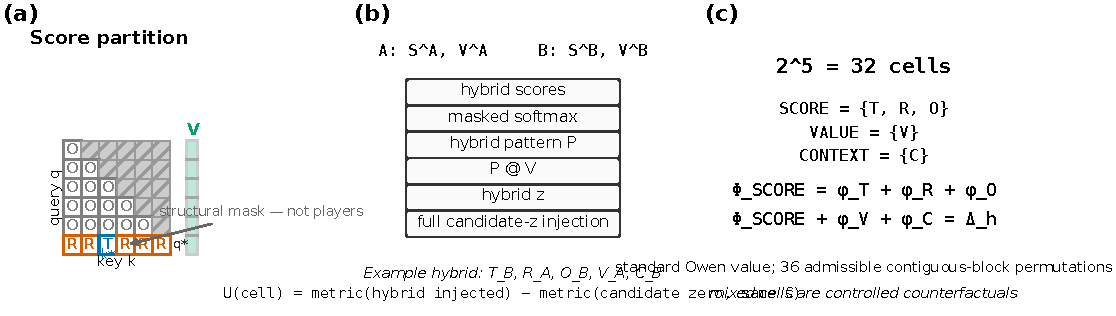
\includegraphics[width=\textwidth]{figures/Fig2.pdf}
\caption{FALI counterfactual intervention game. (a) Structurally valid pre-softmax scores are partitioned into task-target coordinate(s) $T$, rivals $R$ in the same task-relevant query row, and other valid scores $O$; masked coordinates are excluded. (b) Each hybrid cell selects $T,R,O,V,C$ from intact or perturbed endpoints, reconstructs the candidate attention computation, and measures utility relative to a candidate-zero run in the same context. (c) The $2^5=32$ cells are attributed with the standard Owen value under SCORE=$\{T,R,O\}$, VALUE=$\{V\}$, CONTEXT=$\{C\}$, yielding exact coarse--fine reconciliation}
\label{fig:fali-game}
\end{figure*}


\subsection{Owen attribution and coarse--fine reconciliation}\label{sec:owen}

Let the players be $N=\{T,R,O,V,C\}$ and associate each coalition with the corresponding FALI hybrid. We use the standard Owen value with the fixed coalition structure
\begin{equation}
\Pi=\{\mathrm{SCORE}=\{T,R,O\},\;\mathrm{VALUE}=\{V\},\;\mathrm{CONTEXT}=\{C\}\}.
\label{eq:owen-partition}
\end{equation}
This averages marginal contributions over all block-respecting permutations rather than imposing a fixed sequential ordering \citep{owen1977values}. The full expression and equivalent 36-permutation implementation are given in the Supplementary Information.

Two identities are central. First, efficiency allocates the complete endpoint change:
\begin{equation}
\phi_T+\phi_R+\phi_O+\phi_V+\phi_C=\Delta_h.
\label{eq:owen-efficiency}
\end{equation}
Second, the fine score attributions reconcile with the three-player quotient game:
\begin{equation}
\Phi_{\mathrm{SCORE}}=\phi_T+\phi_R+\phi_O,
\label{eq:quotient-consistency}
\end{equation}
while $\phi_V$ and $\phi_C$ equal the VALUE and CONTEXT quotient attributions. These values allocate interaction under the specified game; they are not pure direct effects and need not correspond to unique natural pathways.

The historical two-factor attention-probability formulation is nested as a special case: if the utility is changed to target attention probability, $O,V,C$ are fixed, and only $T$ and $R$ vary, the game reduces to an ordinary two-player Shapley decomposition. The present framework changes both the intervention scope and, crucially, the quantity being explained.
